\documentclass[11pt]{article}

\usepackage{amsmath}
\usepackage{amssymb}
\usepackage[margin=1in]{geometry}
\usepackage{booktabs}
\usepackage{graphicx}
\usepackage{hyperref}
\usepackage{tikz}
\usetikzlibrary{positioning, arrows.meta, fit, backgrounds, calc}

\newcommand{\neuralDMD}{\textsc{NeuralDMD}}
\newcommand{\kine}{\textsc{kine}}
\newcommand{\resolve}{\textsc{resolve}}
\newcommand{\Stokes}{S}
\DeclareMathOperator*{\argmin}{arg\,min}

\title{Polarimetric \neuralDMD:\\
       dynamical modes of a polarized black-hole movie}
\author{}
\date{}

\begin{document}
\maketitle

\begin{abstract}
\neuralDMD{} reconstructs a black-hole movie from sparse interferometric
visibilities as a sum of dynamic modes: a static image plus a handful of complex
spatial modes, each rotating and decaying at its own complex frequency. This note
extends the method to full polarization $(I,Q,U,V)$. The central design question
is how much temporal structure the Stokes parameters should share. We answer it
by measurement rather than assertion: the polarization fields are given access to
a \emph{shared} bank of frequencies alongside \emph{private} modes of their own,
and the fitted amplitudes then report how much of the polarized variability
actually lives on the shared ladder. We also describe the calibration forward
model (station gains applied to the model visibilities, in \resolve{} order
rather than \kine{}'s data-side division) and the priors the objective carries,
separating those that encode physics from those that are tuned by hand.
\end{abstract}

\section{Background: \neuralDMD{} for Stokes $I$}

A dynamic-mode decomposition writes a linear dynamical system as a sum of
separable space--time modes,
\begin{equation}
  I(x,y,t) = \sum_{j=1}^{r} w_j(x,y)\, a_j(t),
  \qquad a_j(t) = b_j e^{\Omega_j t},
  \label{eq:modal}
\end{equation}
with complex eigenvalues $\Omega_j = \alpha_j + i\omega_j$ whose real part sets
the growth or decay rate and whose imaginary part sets the oscillation frequency.
\neuralDMD{} makes every ingredient of Eq.~\eqref{eq:modal} the output of a small
network: a coordinate network $\Theta_w$ maps a positionally-encoded $(x,y)$ to
the spatial modes, and two latent-vector networks $\Theta_\Omega$ and $\Theta_b$
produce the spectrum and the mode amplitudes. Because the image is real, the
implementation carries $r$ \emph{complex} modes and forms
\begin{equation}
  \hat I(x,t) = w_0(x)\, b_0
  \;+\; 2\,\mathrm{Re} \sum_{j=1}^{r} w_j(x)\, b_j\,
        e^{\Omega_j t_{\mathrm{scale}} t},
  \label{eq:dmd}
\end{equation}
the conjugate partners being implicit in the $2\,\mathrm{Re}[\cdot]$. Here
$t \in [0,1]$ is normalized observation time and $t_{\mathrm{scale}} = 200$ puts
the representable rates in a useful range. The spectrum is bounded by
construction, $\alpha_j \le 0$ (no growing modes) and
$\omega_j \in [\omega_{\min}, \omega_{\max}]$.

Two conventions matter below. First, the scale split between $w_j$ and $b_j$ is a
gauge; it is fixed by normalizing each mode to unit RMS over the image, with a
stop-gradient on the norm. This is what makes the amplitudes $|b_j|$ comparable
across modes and across Stokes parameters, and it is what makes any prior on the
amplitude spectrum well posed. Second, the data term is a reduced
$\chi^2$ counted per \emph{real} degree of freedom,
\begin{equation}
  \chi^2 = \frac{\sum_{t,k} m_{tk}\,
                 \bigl| V_{tk} - \hat V_{tk} \bigr|^2 / \sigma_{tk}^2}
                {2 \sum_{t,k} m_{tk}},
  \label{eq:chi2}
\end{equation}
where $m$ is a $0/1$ mask over baselines and the factor $2$ accounts for the real
and imaginary parts of each complex visibility.

\section{Polarization}

\subsection{What has to be represented}

The sky is a Stokes vector $(I,Q,U,V)$ obeying $\sqrt{Q^2+U^2+V^2} \le I$, and
the interferometer with circular feeds measures the correlation products
\begin{equation}
  RR = I + V, \quad LL = I - V, \quad RL = Q + iU, \quad LR = Q - iU .
  \label{eq:circ}
\end{equation}
The linear polarization is naturally a single \emph{complex} field
$P = Q + iU$, of spin weight $2$: under a rotation of the source by an angle
$\phi$, $I$ transforms as a scalar while $P \to e^{2i\phi} P$. The observable
polarization angle is $\chi = \tfrac12 \arg P$.

This spin weight has a direct consequence for the temporal spectrum. If a pattern
rotates rigidly at angular rate $\Omega_{\mathrm{orb}}$, then the azimuthal
Fourier component of order $m$ of $I$ oscillates at $m\,\Omega_{\mathrm{orb}}$,
whereas the order-$m$ component of $P$ oscillates at
$(m-2)\,\Omega_{\mathrm{orb}}$. Intensity and polarization therefore draw their
frequencies from the \emph{same} harmonic ladder while weighting its rungs
differently. A second consequence is that $P$ has a definite sense of rotation:
its temporal spectrum is one-sided, unlike that of the real field $I$, whose
spectrum is conjugate-symmetric by construction.

\subsection{Coordinate charts}

Writing $(Q,U,V)$ directly as free fields satisfies neither $P \le I$ nor the
requirement that polarization vanish where there is no emission. We therefore
build the polarized sky in one of several charts, all of which share the same raw
\neuralDMD{} sub-fields and differ only in the pointwise algebra that turns them
into Stokes parameters (Table~\ref{tab:charts}). The default \emph{fractional}
chart is
\begin{equation}
  Q = m_\ell\, I \cos 2\xi, \qquad
  U = m_\ell\, I \sin 2\xi, \qquad
  V = m_c\, I,
  \label{eq:fractional}
\end{equation}
with $m_\ell = \sigma(\cdot)\,$ bounded in $[0, m_\ell^{\max}]$ and the direction
$(\cos 2\xi, \sin 2\xi)$ normalized to the unit circle, so that
$P = m_\ell |I|$ exactly.

\begin{table}[t]
\centering
\small
\begin{tabular}{llll}
\toprule
chart & construction & $P \le I$ & support \\
\midrule
\texttt{fractional} & $Q,U = m_\ell I(\cos 2\xi, \sin 2\xi)$, unit direction
  & exact & by construction \\
\texttt{direct} & $Q,U$ free signed fields
  & soft penalty & none \\
\texttt{iscaled} & $Q,U = I \tanh(q), I \tanh(u)$
  & $\le \sqrt2 I$ & by construction \\
\texttt{expm} & $(Q,U,V) = I \tanh(p)(q,u,v)/p$
  & exact & by construction \\
\texttt{expm\_full} & $X = \exp M$, $M$ Hermitian (Eq.~\ref{eq:expmfull})
  & exact & by construction \\
\bottomrule
\end{tabular}
\caption{Polarization charts. All consume the same raw sub-fields; only the
pointwise map to Stokes differs. \texttt{expm\_full} parameterizes the full
coherency matrix, so $I>0$ and $P\le I$ hold everywhere, at the cost of making
the intensity logarithmic.}
\label{tab:charts}
\end{table}

The last row of Table~\ref{tab:charts} builds the coherency matrix itself as a
matrix exponential,
\begin{equation}
  X = \exp
  \begin{pmatrix}
    s + v & q + iu \\
    q - iu & s - v
  \end{pmatrix},
  \label{eq:expmfull}
\end{equation}
whose argument is Hermitian, so $X$ is positive semi-definite: $I > 0$ and
$\det X = I^2 - P^2 \ge 0$ hold at every pixel by construction rather than by
penalty. Here $s$ plays the role of a log-intensity.

\subsection{Shared and private temporal modes}

Each raw sub-field is a \neuralDMD{} field of the form of Eq.~\eqref{eq:dmd},
with its own spatial modes $w_j^{\Stokes}$ and amplitudes $b_j^{\Stokes}$. The
design question is whether they should also have their own spectra.

Physics argues for sharing: the frequencies belong to the flow, not to the
observable, so a single orbiting feature should imprint one harmonic ladder on
every Stokes parameter. Statistics argues for sharing too, since the cross-hand
products $RL, LR$ carry a small fraction of the parallel-hand signal-to-noise and
frequencies are the hardest parameters to identify from them. But the spin-2
argument above says the \emph{weights} on that ladder differ between $I$ and $P$,
and nothing guarantees that a real source has no polarization-only variability at
all --- Faraday effects and radially stratified emission can both produce it.

Rather than assume an answer, we make the spectrum a partition. Writing
$\Omega^{\mathrm{shared}}$ for the bank owned by one designated field and
$\Omega^{\Stokes,\mathrm{own}}$ for a field's private spectrum, each coupled field
uses
\begin{equation}
  \Omega^{\Stokes}_j =
  \begin{cases}
    \Omega^{\mathrm{shared}}_j, & j < n_{\mathrm{shared}},\\[2pt]
    \Omega^{\Stokes,\mathrm{own}}_j, & j \ge n_{\mathrm{shared}} .
  \end{cases}
  \label{eq:partition}
\end{equation}
Setting $n_{\mathrm{shared}} = 0$ recovers fully independent fields; setting
$n_{\mathrm{shared}} = r$ shares the whole bank; intermediate values leave each
field private modes. The amplitudes $b_j^{\Stokes}$ are \emph{never} shared,
since the per-Stokes weighting of the harmonics and the relative phases between
Stokes parameters are exactly the physical content we want to measure.

Two coupling scopes are useful. In the first, only the polarization sub-fields
share a bank: $Q$ and $U$ are two components of one spin-2 field, so tying them
together is well motivated independently of what $I$ does. In the second, Stokes
$I$ joins the same bank, which is what makes the mode index $j$ mean the same
frequency in every Stokes parameter and therefore makes per-mode polarimetry well
defined.

Because Eq.~\eqref{eq:partition} leaves private modes available, the fit itself
reports whether they were needed. Define the shared power fraction of a field as
\begin{equation}
  f^{\Stokes}_{\mathrm{shared}}
  = \frac{\sum_{j < n_{\mathrm{shared}}} |b_j^{\Stokes}|^2}
         {\sum_{j} |b_j^{\Stokes}|^2}.
  \label{eq:sharedpower}
\end{equation}
A value near unity says the polarized variability lives on the intensity's
frequency ladder; a small value says it does not, which is a statement about the
source rather than a failure of the fit.

\subsection{Recovering physical rates}

The fitted frequencies are dimensionless. With the normalized time axis spanning
a window of $T$ hours, mode $j$ corresponds to
\begin{equation}
  \omega_j^{\mathrm{phys}} = \frac{\omega_j\, t_{\mathrm{scale}}}{T}
  \quad [\mathrm{rad\ hr^{-1}}],
  \label{eq:physfreq}
\end{equation}
so that an orbital period $T_{\mathrm{orb}}$ appears at
$2\pi / T_{\mathrm{orb}}$ together with its harmonics. Because
$\omega_j \ge 0$ and the conjugate partners are implicit in
Eq.~\eqref{eq:dmd}, the \emph{sense} of rotation is not encoded in the spectrum:
it lives in the azimuthal phase gradient of $\arg w_j(x)$, and any claim about
the direction of motion must be read from the spatial modes rather than from
$\Omega$.

\section{Measurement model}

Model visibilities are formed by sampling the Fourier transform of each Stokes
cube at the observed baselines, combining them into correlation products via
Eq.~\eqref{eq:circ}, and then applying the instrument. For station-based
complex gains $g$, the product $p$ on baseline $(i,j)$ becomes
\begin{equation}
  \hat V^{p}_{ij}(t) \;\longleftarrow\;
  g_{h_i, i}(t)\, \hat V^{p}_{ij}(t)\, \overline{g_{h_j, j}(t)},
  \label{eq:rime}
\end{equation}
where $h_i, h_j$ select the polarization hand appropriate to the product
($RR \to (R,R)$, $RL \to (R,L)$, and so on). Two choices are deliberate. The
gains are applied to the \emph{model} rather than divided into the data: the two
are equivalent for pure gains but only the former remains correct once
leakage terms enter the chain. And the amplitudes are bounded smoothly,
$|g| = g_{\mathrm{lo}} + (g_{\mathrm{hi}}-g_{\mathrm{lo}})\,\sigma(\cdot)$, with
per-station bounds taken from that station's known calibration quality, so a gain
that reaches its bound can still return; a hard clip would zero the gradient
there. Phases are referenced to a fixed station, removing the degeneracy between
a global phase and a shift of the image.

\section{The objective, and which parts of it are priors}

The quantity minimized is
\begin{equation}
  \mathcal{L} = \sum_{p} \chi^2_p
    \;+\; \sum_{k} \lambda_k \, R_k ,
  \label{eq:total}
\end{equation}
with $\chi^2_p$ the reduced $\chi^2$ of Eq.~\eqref{eq:chi2} for each correlation
product and $R_k$ a set of penalties. Amplitude and closure-phase $\chi^2$ are
computed but never enter $\mathcal{L}$; they are diagnostics, and the closure
quantities double as a calibration canary because they are gain-invariant.

It is worth being explicit about how much of Eq.~\eqref{eq:total} is not data.
Table~\ref{tab:priors} sorts the terms by the kind of justification each has. We
distinguish priors that are structural (a physical constraint the parameterization
or the architecture enforces, with no free weight), measured (a number estimated
from the data itself), and hand-tuned (a weight chosen because it worked). The
last category is the one to minimize, and the training loop records every term's
value so that the balance between data and prior is a measured number for every
run rather than an inference from the configuration file.

\begin{table}[t]
\centering
\small
\begin{tabular}{lll}
\toprule
term & kind & justification \\
\midrule
$\alpha_j \le 0$, $\omega_j$ bounded & structural & no growing modes; band limit \\
unit-RMS mode gauge & structural & removes the $w \leftrightarrow b$ scale freedom \\
$P \le I$, support & structural & enforced by the chart (Table~\ref{tab:charts}) \\
negativity of $I$ & structural & $\lambda$ fixed, penalizes $I<0$ only \\
shared/private spectrum & structural & Eq.~\eqref{eq:partition}; no weight \\
total flux anchor & measured & zero-spacing flux from intra-site baselines \\
station gain bounds & measured & per-station calibration quality \\
compactness, $L_1$ sparsity & hand-tuned & weights chosen empirically \\
\bottomrule
\end{tabular}
\caption{The objective's ingredients, sorted by how each is justified. The aim of
this work is to move terms up this table --- to replace tuned weights by
structure the model carries for a stated reason.}
\label{tab:priors}
\end{table}

\section{Architecture}

\begin{figure}[t]
\centering
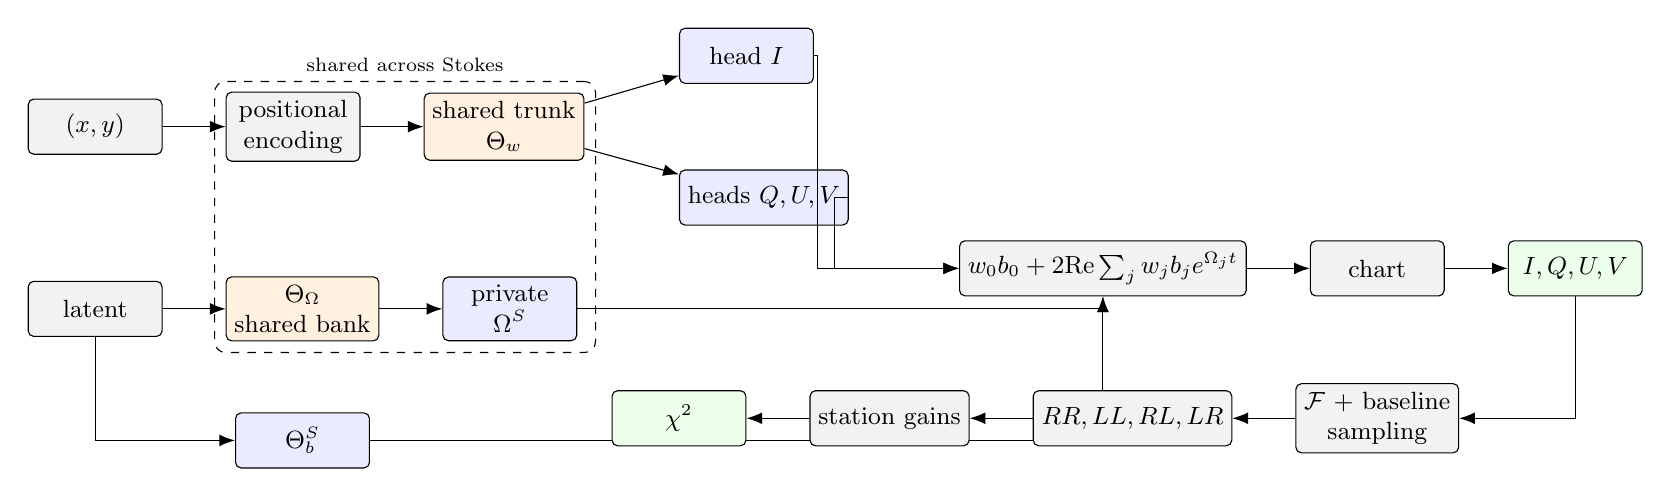
\begin{tikzpicture}[
    font=\small,
    box/.style={draw, rounded corners=2pt, minimum height=7mm, minimum width=17mm,
                align=center, inner sep=3pt},
    net/.style={box, fill=blue!8},
    op/.style={box, fill=black!5},
    res/.style={box, fill=green!8},
    sh/.style={box, fill=orange!12},
    ar/.style={-{Latex[length=2mm]}, thin},
    node distance=5mm and 8mm,
  ]

  % ---- spatial branch
  \node[op] (xy) {$(x,y)$};
  \node[op, right=of xy] (enc) {positional\\encoding};
  \node[sh, right=of enc] (trunk) {shared trunk\\$\Theta_w$};
  \node[net, right=12mm of trunk, yshift=9mm] (headI) {head $I$};
  \node[net, right=12mm of trunk, yshift=-9mm] (headP) {heads $Q,U,V$};

  \draw[ar] (xy) -- (enc);
  \draw[ar] (enc) -- (trunk);
  \draw[ar] (trunk) -- (headI);
  \draw[ar] (trunk) -- (headP);

  % ---- temporal branch
  \node[op, below=16mm of xy] (lat) {latent};
  \node[sh, right=of lat] (om) {$\Theta_\Omega$\\shared bank};
  \node[net, right=of om] (priv) {private\\$\Omega^{\Stokes}$};
  \node[net, below=9mm of om] (bnet) {$\Theta_b^{\Stokes}$};

  \draw[ar] (lat) -- (om);
  \draw[ar] (om) -- (priv);
  \draw[ar] (lat) |- (bnet);

  % ---- combine
  \node[op, right=14mm of headP, yshift=-9mm] (sum)
    {$w_0 b_0 + 2\mathrm{Re}\sum_j w_j b_j e^{\Omega_j t}$};
  \node[op, right=of sum] (chart) {chart};
  \node[res, right=of chart] (cubes) {$I,Q,U,V$};

  \draw[ar] (headI) -- ++(9mm,0) |- (sum);
  \draw[ar] (headP) -- ++(9mm,0) |- (sum);
  \draw[ar] (priv) -| (sum);
  \draw[ar] (bnet) -| (sum);
  \draw[ar] (sum) -- (chart);
  \draw[ar] (chart) -- (cubes);

  % ---- measurement
  \node[op, below=11mm of chart] (ft) {$\mathcal{F}$ + baseline\\sampling};
  \node[op, left=of ft] (prod) {$RR,LL,RL,LR$};
  \node[op, left=of prod] (gain) {station gains};
  \node[res, left=of gain] (chi) {$\chi^2$};

  \draw[ar] (cubes) |- (ft);
  \draw[ar] (ft) -- (prod);
  \draw[ar] (prod) -- (gain);
  \draw[ar] (gain) -- (chi);

  \begin{scope}[on background layer]
    \node[draw, dashed, rounded corners, fit=(trunk)(om),
          inner sep=4pt, label={[font=\scriptsize]above:shared across Stokes}] {};
  \end{scope}
\end{tikzpicture}
\caption{Polarimetric \neuralDMD{}. Coordinates pass through a positional
encoding and a spatial trunk to per-Stokes mode heads; a latent vector drives the
temporal spectrum and the per-Stokes amplitudes. The dashed region marks what may
be shared between Stokes: the temporal bank always, the spatial trunk optionally.
Private spectra remain available so a Stokes parameter can carry a frequency the
others do not. The reconstructed cubes are pushed through the chart, Fourier
transformed and sampled at the observed baselines, combined into correlation
products, and corrupted by station gains before comparison with the data.}
\label{fig:arch}
\end{figure}

\begin{figure}[t]
\centering
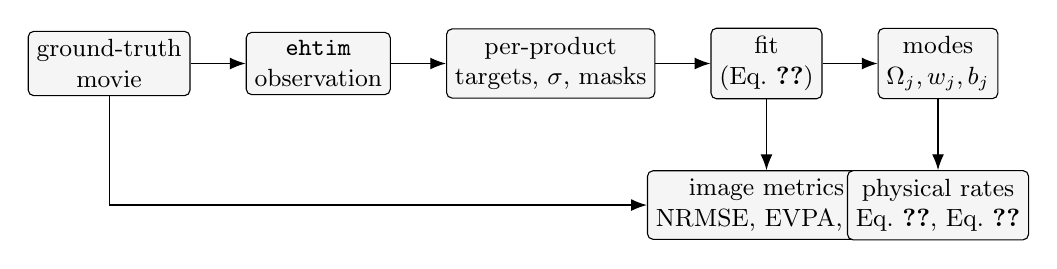
\begin{tikzpicture}[
    font=\small,
    stg/.style={draw, rounded corners=2pt, minimum height=7mm, align=center,
               inner sep=3pt, fill=black!4},
    ar/.style={-{Latex[length=2mm]}, thin},
    node distance=5mm and 7mm,
  ]
  \node[stg] (truth) {ground-truth\\movie};
  \node[stg, right=of truth] (obs) {\texttt{ehtim}\\observation};
  \node[stg, right=of obs] (prod) {per-product\\targets, $\sigma$, masks};
  \node[stg, right=of prod] (fit) {fit\\(Eq.~\ref{eq:total})};
  \node[stg, right=of fit] (mod) {modes\\$\Omega_j, w_j, b_j$};

  \node[stg, below=9mm of fit] (img) {image metrics\\NRMSE, EVPA, $\beta_2$};
  \node[stg, below=9mm of mod] (phys) {physical rates\\Eq.~\ref{eq:physfreq}, Eq.~\ref{eq:sharedpower}};

  \draw[ar] (truth) -- (obs);
  \draw[ar] (obs) -- (prod);
  \draw[ar] (prod) -- (fit);
  \draw[ar] (fit) -- (mod);
  \draw[ar] (fit) -- (img);
  \draw[ar] (mod) -- (phys);
  \draw[ar] (truth) |- (img);
\end{tikzpicture}
\caption{Evaluation pipeline. A ground-truth movie (parametric or from the EHT
validation ladder) is observed with the array's real coverage, ingested into
per-product visibilities, and fitted. The reconstruction is scored against the
truth in the image domain, while the recovered modes are scored against the
physical rates that generated the movie.}
\label{fig:pipeline}
\end{figure}

\section{Results}

\emph{[Filled from the completed sweeps; see the accompanying tables.]}

\section{Relation to other methods}

\kine{} also represents a movie with a coordinate network and also solves station
gains, but it fixes Stokes $I$ first and then fits polarization on the frozen
result. That ordering forecloses a joint solution for leakage terms, which
requires the total intensity and the polarization to move together. Its published
description also understates its priors: the released implementation carries
penalties on the outer field of view, on the light curve, on the static and
dynamic flux separately, on persistent flux in the dynamic component, and a
support term that penalizes polarized flux where the intensity is faint --- the
last of which is functionally identical to a term we arrived at independently.

\resolve{} takes the opposite stance, treating the reconstruction as Bayesian
inference under explicit priors, and does solve calibration and leakage jointly.
Its strength is precisely the weight of those priors. The contribution we can
make is therefore neither joint calibration nor prior engineering, but the
explicit mode representation: a spectrum $\{\Omega_j\}$ with per-Stokes
amplitudes that can be compared directly against the rates of change in the
source, which neither method produces.

\end{document}
